\chapter{Conception, Modélisation et Architecture }
\label{chap:deuxiemechapitre}


\section{Introduction du chapitre}

Ce chapitre traduit les enjeux métier en spécifications techniques et présente l'architecture du système. Nous formalisons d'abord les besoins fonctionnels et non fonctionnels, puis proposons une modélisation UML des interactions. Enfin, nous décrivons l'architecture basée sur la séparation entre SAP Commerce et le microservice d'intelligence artificielle.

\section{Spécification des besoins}

Dans cette section, nous formalisons les exigences du système en distinguant les besoins fonctionnels, qui décrivent les services attendus et les besoins non fonctionnels, qui définissent les contraintes de qualité et de performance. Cette étape permet de traduire les attentes métier en spécifications exploitables pour la conception.

\subsection{Identification des acteurs}

Tout système interactif repose sur une ou plusieurs catégories d'utilisateurs. Identifier précisément ces acteurs permet de définir les fonctionnalités attendues.

\subsubsection{Le responsable de l'enrichissement du produit}

L'utilisateur principal du système est le responsable de l'enrichissement du produit. Il intervient dans la gestion, l'amélioration et la validation des fiches des produits au sein de SAP Commerce. Il crée, modifie ou valide régulièrement les données des produits avant leur publication. 

Son rôle consiste à garantir la qualité et la complétude des informations des produits. Le système proposé l'assiste en générant automatiquement des enrichissements et en signalant les anomalies détectées. Cependant, le responsable de l'enrichissement du produit conserve l'autorité finale : il examine les propositions du système et approuve ou rejette chaque suggestion en fonction de son jugement professionnel.

\subsection{Recueil des besoins fonctionnels}

Les besoins fonctionnels décrivent les actions que le responsable de l'enrichissement du produit doit pouvoir accomplir au travers du système. Ils structurent l'interaction entre l'utilisateur et la solution.

\subsubsection{Enrichissement des contenus des produits}

Le responsable de l'enrichissement du produit doit pouvoir consulter les enrichissements générés automatiquement par le système pour chaque produit. Ces enrichissements incluent :

\begin{itemize}
    \item une description détaillée conçue pour présenter les caractéristiques principales du produit 
    \item un résumé court destiné à une présentation rapide sur les interfaces compactes 
    \item les traductions des contenus dans les langues demandées
\end{itemize}

Ces propositions doivent être clairement présentées dans l'interface de SAP Commerce Backoffice, permettant au Responsable de l'enrichissement du produit d'accepter, modifier ou rejeter chaque suggestion.

\subsubsection{Détection des anomalies}

Le système doit identifier automatiquement les problèmes présents dans les données des produits. Cela inclut :

\begin{itemize}
    \item les champs obligatoires absents ou non conformes aux règles définies 
    \item les erreurs de structure ou de format 
    \item les incohérences sémantiques ou linguistiques 
\end{itemize}

Cette détection permet au responsable de l'enrichissement du produit de corriger les défauts avant la publication et d'améliorer la qualité globale du catalogue.

\subsubsection{Validation des fiches des produits}

Le responsable de l'enrichissement du produit doit pouvoir consulter un score de qualité global pour chaque fiche du produit, accompagné d'une liste des anomalies détectées. Ce score synthétise les résultats de l'analyse technique et sémantique. Sur cette base, Le responsable de l'enrichissement du produit décide d'approuver la fiche ou d'exiger des corrections avant publication.
\subsection{Recueil des besoins non fonctionnels}
Les besoins non fonctionnels définissent les critères de qualité que doit respecter le système afin de garantir son efficacité, sa fiabilité et son intégration dans l'environnement existant. Ils concernent notamment les aspects liés à la performance, la sécurité, l'utilisabilité et la maintenabilité de la solution.
\newpage
\subsubsection{Fiabilité}

Le système doit fournir des enrichissements et des validations de qualité suffisante. Cette fiabilité repose sur des règles métier bien définies, des modèles adaptés au domaine et une validation humaine des résultats proposés.

\subsubsection{Performance}

Le temps de réponse doit être acceptable pour ne pas interrompre le flux de travail du responsable de l'enrichissement du produit. Une architecture découplée, avec l'intelligence artificielle déployée dans un microservice externe, permet d'optimiser les temps de traitement sans ralentir la plateforme SAP Commerce.

\subsubsection{Sécurité}

La sécurité est assurée par la protection des données échangées entre SAP Commerce et le microservice d'intelligence artificielle. Seules les informations nécessaires aux traitements d'enrichissement et de validation sont transmises afin de limiter l'exposition des données sensibles. Les échanges sont sécurisés via HTTPS et authentifiés pour garantir que seules les requêtes légitimes sont traitées par le microservice.

\subsubsection{Utilisabilité}

Les résultats d'enrichissement et de validation doivent être présentés de manière claire et compréhensible dans l'interface du Backoffice. Le responsable de l'enrichissement du produit doit rapidement identifier les anomalies signalées et les enrichissements proposés, afin de pouvoir les accepter ou rejeter.

\subsubsection{Maintenabilité}

L'architecture doit permettre une évolution indépendante du microservice d'intelligence artificielle sans impacter SAP Commerce. Les règles métier et les modèles doivent pouvoir être actualisés sans modifier la plateforme e-commerce existante.


\section{Modélisation des besoins}

Cette section modélise le système d'enrichissement et de validation des produits au travers de trois diagrammes UML complémentaires : le diagramme de cas d'utilisation expose les scénarios métier, le diagramme de séquence détaille l'orchestration temporelle des échanges et le diagramme d'activités synthétise le flux de contrôle du traitement.
\newpage
\subsection{Diagramme de cas d'utilisation}

Le diagramme de cas d'utilisation présente les interactions principales entre le responsable de l'enrichissement du produit et le système. Il met en évidence les fonctionnalités offertes par la solution : l'enrichissement automatique des contenus, la détection des anomalies, la consultation des résultats de validation et la prise de décision finale avant publication. Ces interactions sont illustrées dans la Figure~\ref{fig:usecase}.

\begin{figure}[H]
    \centering
    
\includegraphics[width=1\textwidth]{usecase.png}
    \caption{Diagramme de cas d'utilisation}
    \label{fig:usecase}
\end{figure}

Ce diagramme montre que le responsable conserve un rôle central de décideur, tandis que les traitements techniques (enrichissement et validation) sont automatisés par la solution.
\newpage
\subsection{Diagramme de séquence}

Le diagramme de séquence détaille l'ordre temporel des interactions entre les différents acteurs du système. La Figure~\ref{fig:sequence} illustre le flux complet d'une requête depuis sa création dans SAP Commerce jusqu'à la réception de la réponse du microservice d'intelligence artificielle.

\begin{figure}[H]
    \centering
    
\includegraphics[width=1.09\textwidth]{sequence01.png}
    \caption{Diagramme de séquence}
    \label{fig:sequence}
\end{figure}

Ce diagramme démontre la nature asynchrone et bien définie des échanges : chaque acteur (responsable, SAP Commerce, microservice) exécute ses responsabilités de manière séquentielle, facilitant ainsi le débogage et l'optimisation du système.

\subsection{Diagramme d'activités}

Le diagramme d'activités représente le flux global du traitement d'une fiche du produit et met en évidence les différentes étapes ainsi que les points de décision du processus. Il illustre l'enchâinement entre l'intervention du responsable de l'enrichissement du produit, l'orchestration réalisée par SAP Commerce, les traitements effectués par le microservice d'intelligence artificielle et la décision finale avant publication. Ce flux complet est présenté dans la Figure~\ref{fig:activities}.



\begin{figure}[H]
    \centering
    
\includegraphics[width=0.9\textwidth]{activités.png}
    \caption{Diagramme d'activités}
    \label{fig:activities}
\end{figure}

Ce diagramme souligne l'importance de la validation humaine dans le processus : bien que le système automatise les taches d'enrichissement et de validation technique, la décision finale de publication demeure sous le contrôle du responsable, garantissant ainsi une qualité finale acceptable par le métier.

\newpage
\section{Architecture globale}

L'architecture du système repose sur une séparation de responsabilités entre la plateforme SAP Commerce et un microservice d'intelligence artificielle indépendant. Cette approche permet de centraliser les traitements intelligents dans un composant dédié tout en intégrant les résultats dans le workflow existant de gestion des produits. L'organisation globale de cette architecture est illustrée dans la Figure~\ref{fig:architecture_globale}.

\subsection{Vue générale de l'architecture}

L'architecture repose sur trois éléments principaux : SAP Commerce qui orchestre le processus métier et accueille les extensions nécessaires au déclenchement des traitements, une API REST qui assure la communication entre les deux systèmes  et un microservice d'intelligence artificielle externe, qui réalise les traitements d'enrichissement et de validation.

Cette approche présente plusieurs avantages. Elle concentre les traitements intelligents dans un composant indépendant, facilitant la maintenance et l'évolution de la solution. Elle permet également une séparation claire des responsabilités : SAP Commerce gère le cycle de vie des produits tandis que le microservice d'intelligence artificielle prend en charge les traitements liés à l'intelligence artificielle.

\begin{figure}[H]
    \centering
    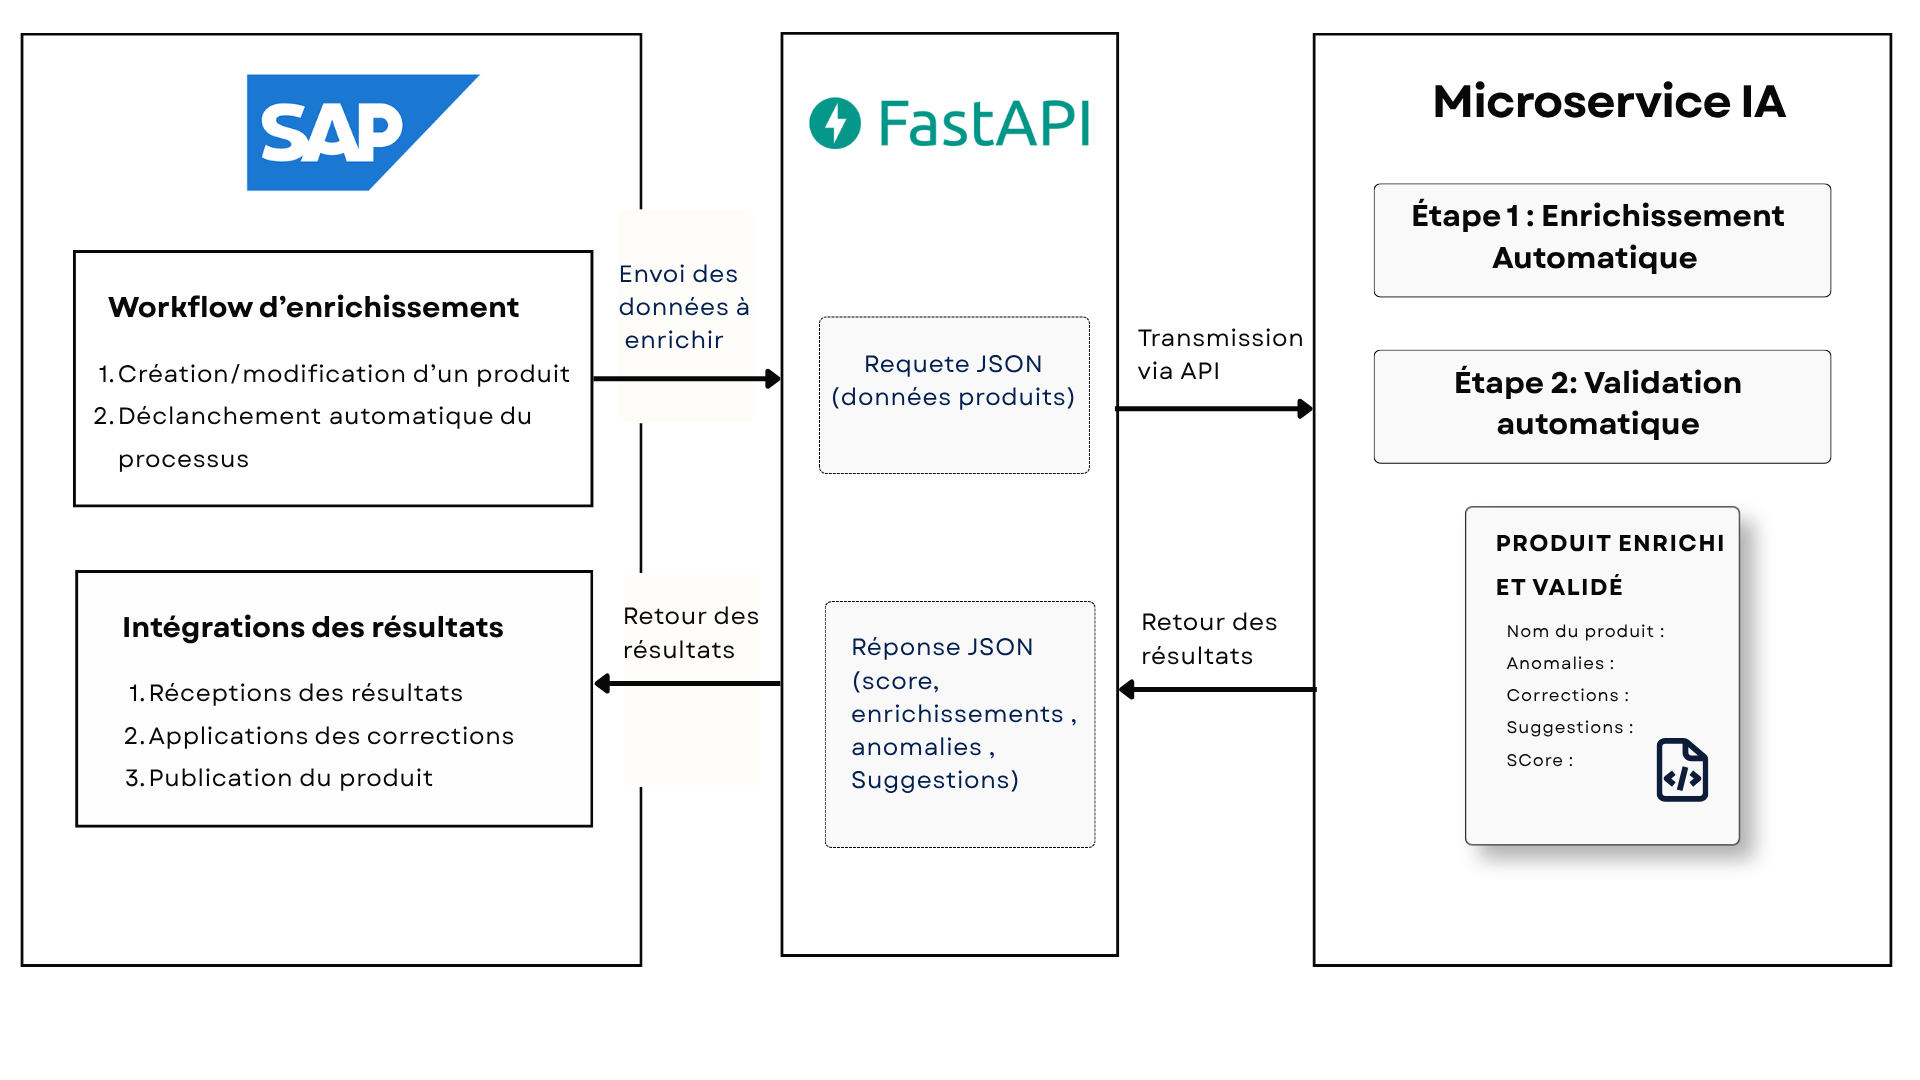
\includegraphics[width=1\textwidth]{images/architecture.png}
    \caption{Vue d'ensemble de l'architecture du système d'enrichissement intelligent}
    \label{fig:architecture_globale}
\end{figure}
Cette architecture démontre l'efficacité d'une séparation nette entre la gestion transactionnelle (SAP Commerce) et les traitements intelligents (microservice). Cette approche facilite la maintenance, l'amélioration et le déploiement de chaque composant indépendamment, tout en garantissant une intlégration harmonieuse au sein de l'ecosystème global.\newpage

\subsection{Description détaillée des composants}

\subsubsection{SAP Commerce : orchestrateur métier}

SAP Commerce (anciennement Hybris) constitue le cœur du système de gestion des produits. Elle assure la gestion des données produits et l'orchestration du workflow associé.

SAP Commerce accueille les événements métier relatifs à la création et la modification de produits. Des actions et services workflow ont été ajoutés pour intégrer le traitement d'enrichissement et de validation dans ce flux existant. Lorsque le responsable de l'enrichissement du produit crée ou modifie une fiche du produit, un événement déclenche l'extraction des données pertinentes (titre, description, attributs, catégorie, langue). Ces données sont nettoyées, normalisées et structurées en JSON pour transmission au microservice. À réception des résultats d'analyse, SAP Commerce les présente au responsable de l'enrichissement du produit dans l'interface du Backoffice. Le responsable de l'enrichissement du produit examine alors les enrichissements proposés, les anomalies signalées et le score de qualité, puis prend la décision d'approuver ou de corriger la fiche avant publication.

\subsubsection{API REST : contrat d'intégration}

L'API REST assure la communication standardisée entre SAP Commerce et le microservice d'intelligence artificielle. REST a été choisi car c'est un standard pour les intégrations inter-services : simple à mettre en œuvre, adapté aux requêtes synchrones et bien supporté par les frameworks modernes.

Les données sont échangées au format JSON. Les réponses structurées en JSON contiennent : les enrichissements générés, la liste des anomalies détectées et un score de qualité global.

\subsubsection{Microservice d'intelligence artificielle : traitements d'enrichissement et de validation}

Le microservice d'intelligence artificielle, développé avec FastAPI et Python, implémente les traitements d'enrichissement et de validation des produits. Il fonctionne selon deux phases successives : l'enrichissement d'abord, puis la validation. Cette séparation permet une progression claire du traitement et facilite le diagnostic en cas de dysfonctionnement.

\subsection{Communication entre SAP Commerce et le microservice}

La communication entre SAP Commerce et le microservice d'intelligence artificielle repose sur une API REST utilisant le format JSON. SAP Commerce transmet uniquement les informations nécessaires aux traitements d'enrichissement et de validation, afin de limiter l'exposition des données sensibles.

Le microservice reçoit ces données structurées, exécute les traitements demandés, puis retourne une réponse contenant les contenus enrichis, les anomalies détectées et le score de qualité associé.
\newpage
\subsection{Flux global de traitement}

Le fonctionnement global de la solution repose sur l'échange entre SAP Commerce et le microservice d'intelligence artificielle. Le traitement d'une fiche du produit suit les étapes techniques suivantes :

\begin{enumerate}

\item \textbf{Préparation des données :} SAP Commerce récupère les informations nécessaires depuis la fiche du produit et prépare une structure JSON conforme au contrat défini avec le microservice d'intelligence artificielle.

\item \textbf{Transmission au microservice d'intelligence artificielle :} Les données préparées sont envoyées via une requête REST afin de déclencher les traitements d'intelligence artificielle.

\item \textbf{Traitement d'enrichissement :} Le microservice génère les contenus attendus, notamment la description détaillée, le résumé court et les traductions demandées.

\item \textbf{Traitement de validation :} Après enrichissement, le système analyse la qualité des contenus selon des règles techniques et sémantiques, puis identifie les anomalies éventuelles.

\item \textbf{Retour et intégration des résultats :} Le microservice retourne les résultats sous forme structurée. SAP Commerce présente ces informations dans le Backoffice afin de permettre au responsable de l'enrichissement du produit d'effectuer la validation finale.

\end{enumerate}

Cette communication assure une séparation claire entre la gestion métier des produits dans SAP Commerce et les traitements intelligents réalisés par le microservice d'intelligence artificielle.


\subsection{Justification des choix architecturaux}

Cette architecture a été retenue pour plusieurs raisons.

\subsubsection{Intégration progressive dans l'existant} Plutôt que de remplacer le workflow produit existant, l'architecture ajoute des extensions minimales dans SAP Commerce pour déclencher les traitements IA. Cette approche réduit le risque de perturbation du système en production.

\subsubsection{Indépendance des évolutions} Le microservice peut être amélioré ou modifié sans impact sur le workflow SAP Commerce. Les règles métier et les modèles peuvent être actualisés indépendamment.

\subsubsection{Traçabilité des traitements} Les échanges entre les deux systèmes sont loggés, permettant de suivre chaque traitement et de diagnostiquer les dysfonctionnements.

\subsubsection{Responsabilité humaine préservée} Le responsable de l'enrichissement du produit conserve l'autorité finale sur la publication des fiches, garantissant un contrôle qualité manuel sur les décisions critiques.

\subsection{Justification des choix technologiques}

\subsubsection{SAP Commerce} L'équipe utilise SAP Commerce pour gérer le catalogue e-commerce. Cette plateforme offre le workflow produit, les événements métier et les APIs nécessaires à l'intégration.

\subsubsection{FastAPI et Python} FastAPI est un framework léger et performant pour construire des APIs. Python offre des bibliothèques matures pour le traitement du texte et l'intégration de modèles de traitement naturel du langage, facilitant le développement rapide des traitements IA.

\subsubsection{REST et JSON} REST est le standard pour les communications inter-services. JSON offre un format léger et universel pour l'échange de données structurées.
\vspace{0.2cm}

Chaque choix correspond à une nécessité du projet et aux contraintes d'intégration avec les systèmes existants.

\section{Conclusion du chapitre}

Ce chapitre a présenté la conception et l'architecture du système d'enrichissement intelligent. Nous avons formalisé les besoins fonctionnels et non fonctionnels, modélisé les interactions par des diagrammes UML et décrit l'architecture distribuée reposant sur SAP Commerce et un microservice d'intelligence artificielle externe. Cette séparation des responsabilités garantit la stabilité du système existant tout en permettant l'évolution indépendante des composants IA.

Le chapitre suivant décrit la réalisation concrète : implémentation du microservice, intégration avec SAP Commerce, résultats obtenus.





